In this section, we will prove \Cref{thm:filt-bound-finale}, which we used in \Cref{sec:Finale} to prove \Cref{thm:intro-main}. That is to say, we provide for each prime $p$ a bound on the $\HFp$-Adams filtration of the Toda bracket $w$ of \Cref{lem:toda-main}.

To accomplish this, we will lift the Toda bracket along the functor \[ \tau^{-1} : \mathrm{Syn}_{\HFp} \to \Sp\] in such a way that \Cref{cor:synth-filt} implies the existence of the desired bound on the $\HFp$-Adams filtration.

The first ingredient that we will need is a bound on the $\HFp$-Adams filtration of the map \[J : \Sigma^{\infty} \Oo\mathrm{\langle4n-1 \rangle} \to \Ss,\] at least when restricted to a skeleton of $\Sigma^{\infty} \Oo\mathrm{\langle 4n-1 \rangle}$. We must restrict to a skeleton because the map $J$ does not otherwise have high $\HFp$-Adams filtration.

\begin{cnv}
In the remainder of this section, we fix a prime $p$ and implicitly $p$-complete all spectra. Furthermore, all synthetic spectra will be taken with respect to $\HFp$.
\end{cnv}
\todo{Jeremy: Check numbers in this section.}

\begin{rmk}
 Recall from Definition \ref{dfn:skeleton} that
	$$M \longrightarrow \Sigma^{\infty} \Oo \mathrm{\langle 4n-1 \rangle}$$
	denotes the inclusion of an $(8n-1)$-skeleton of $\Sigma^{\infty} \Oo \mathrm{\langle 4n-1 \rangle}$. In particular, the induced map
	$$\mathrm{H}_*(M;\F_p) \longrightarrow \mathrm{H}_*(\Sigma^{\infty} \Oo \mathrm{\langle 4n-1 \rangle};\F_p)$$
is an isomorphism for $* < 8n-1$ and a surjection for $* = 8n-1$, and $\mathrm{H}_*(M;\F_p) \cong 0$ for $* > 8n-1$.
\end{rmk}

\begin{ntn}
    Let $h(k)$ denote the number of integers $0 < s \leq k$ which are congruent to one of $0,1,2$ or $4$ mod $8$. Then we set \[N_2 = h(4n-1) - \lfloor \log_2 (8n) \rfloor + 1\] and, for $p$ odd, \[N_p = \left\lfloor \frac{4n}{2p-2} \right\rfloor - \left\lfloor \log_p (4n) \right\rfloor.\] Note that this notation suppresses the dependence of $N_2$ and $N_p$ on $n$.
\end{ntn}

\begin{lem}\label{lemm:filtration}
The $\HFp$-Adams filtration of the composite map of spectra
	$$M \longrightarrow \Sigma^{\infty} \Oo \mathrm{\langle 4n-1 \rangle} \stackrel{J}{\longrightarrow} \mathbb{S}$$
	is at least $N_p$.
\end{lem}

We will prove \Cref{lemm:filtration} in \Cref{subsec:filtration}.
Using \Cref{lemm:filtration}, we proceed to construct a lift of the diagram defining the Toda bracket $w$ to $\mathrm{Syn}_{\HFp}$.
We take the first step of this construction below:

\begin{cnstr}
By \Cref{lemm:adams-fil1}, \Cref{lemm:filtration} implies the existence of a factorization in $\mathrm{Syn}_{\HFp}$
\begin{center}
  \begin{tikzcd}
    & \arrow{d}{\tau^{N_p}} \Ss^{0,-N_p} \\
    \nu M \arrow[dashed]{ur} \arrow{r}{J} & \Ss^{0,0},
  \end{tikzcd}
\end{center}
which we will prefer to view as a morphism
$$\wt{J}:\Sigma^{0,N_p}\nu M \longrightarrow \Ss^{0,0}.$$
As in \Cref{dfn:skeleton}, we view $x$ as an element of $\pi_{4n-1} M$.
We may then obtain a class $y$ as the composition
$$ y:\Ss^{4n-1,4n+N_p-1} \xrightarrow{\nu(x)} \Sigma^{0,N_p} \nu M \xrightarrow{\wt{J}} \Ss^{0,0}. $$
This element $y$ is a member of the bigraded homotopy group $\pi_{4n-1,4n+N_p-1}\Ss^{0,0}$.
\end{cnstr}

Before constructing our lift of the Toda bracket $w$ we reproduce the relevant diagram, which appeared in Lemma \ref{lem:toda-main}, for the convenience of the reader.
\begin{center}
  \begin{tikzcd}[column sep = huge]
    \mathbb{S}^{8n-2} \arrow{r}{2}
    \arrow[rrdd, bend right=20,""{name=D}] \arrow[rrdd, bend right=20,swap,"0"] \arrow[rr,bend left = 30,""{name=U},"0"]
    \arrow[rrdd, bend right=20,""{name=D}] \arrow[rrdd, bend right=20,swap,"0"] \arrow[rr,bend left = 30,""{name=U},"0"]
    & \mathbb{S}^{8n-2} \arrow[Leftrightarrow, from=D, "h"] \arrow[Leftrightarrow, from=U, "f"] \arrow{r}{xJ(x)} \arrow[rdd,""{name=MU},"J(x)^2" description] \arrow[rdd,swap, ""{name=MD},"J(x)^2" description]
    & M \arrow{dd}{J}  \arrow[bend left=20,Leftrightarrow, from=MU, swap, "g"] \\ \\
    & & \mathbb{S}.
  \end{tikzcd}
\end{center}
The homotopies $f,g$ and $h$ are chosen as follows:
\begin{itemize}
\item $f$ is an arbitrary nullhomotopy.
\item $g$ is the canonical homotopy associated to the fact that $J$ is a map of $\Ss$-modules.
\item $h$ is the canonical nullhomotopy given by the $\mathbb{E}_\infty$-ring structure on $\Ss$.
\end{itemize}

\begin{cnstr}\label{cnstr:synth-toda-diagram}
  We may form the following diagram of morphisms and homotopies in $\Syn_{\HFp}$
\begin{center}
  \begin{tikzcd}[column sep = huge]
    \mathbb{S}^{8n-2,8n+2N_p-2} \arrow{r}{2}
    \arrow[rrdd, bend right=20,""{name=D}] \arrow[rrdd, bend right=20,swap,"0"] \arrow[rr,bend left = 30,""{name=U},"0"]
    \arrow[rrdd, bend right=20,""{name=D}] \arrow[rrdd, bend right=20,swap,"0"] \arrow[rr,bend left = 30,""{name=U},"0"]
    & \mathbb{S}^{8n-2,8n+2N_p-2} \arrow[Leftrightarrow, from=D, "\tilde{h}"] \arrow[Leftrightarrow, from=U, "\tilde{f}"] \arrow{r}{\nu(x)y} \arrow[rdd,""{name=MU},"y^2" description]
    & \Sigma^{0,N_p}\nu(M) \arrow{dd}{\wt{J}}  \arrow[swap,Leftrightarrow, from=MU,"\tilde{g}"] \\ \\
    & & \Ss^{0,0}, 
  \end{tikzcd}
\end{center}
where the homotopies $\tilde{f},\tilde{g}$ and $\tilde{h}$ are chosen as follows:
\begin{itemize}
\item $\tilde{f}$ is an arbitrary nullhomotopy, which exists as a consequence of \Cref{thm:vanishinggroup}.
\item $\tilde{g}$ is the canonical homotopy that expresses the fact that $\tilde{J}$ is a map of right $\Ss^{0,0}$-modules.
\item $\tilde{h}$ is the canonical nullhomotopy that comes from the fact that $\Ss^{0,0}$ is an $\mathbb{E}_\infty$-ring in the symmetric moniodal $\infty$-category $\mathrm{Syn}_{\HFp}$.
\end{itemize}

    %% We set $\tilde{h}$ to be the canonical nullhomotopy that comes from the fact that $\Ss^{0,0}$ is an $\mathbb{E}_\infty$-ring in the symmetric moniodal $\infty$-category $\mathrm{Syn}_{\HFp}$. The homotopy $\tilde{g}$ is the canonical homotopy that expresses the fact that $\tilde{J}$ is a map of right $\Ss^{0,0}$-modules.  The homotopy $\tilde{f}$ is a completely arbitrary nullhomotopy, which exists as a consequence of the following proposition. 
\end{cnstr}

\begin{prop}\label{thm:vanishinggroup}
    The bigraded homotopy group $\pi_{8n-2,8n+N_p-2}(\nu M )$ is trivial for $n \geq 3$.
\end{prop}

We will prove \Cref{thm:vanishinggroup} in \Cref{subsec:vanishinggroup}. By construction, the diagram of \Cref{cnstr:synth-toda-diagram} maps under the symmetric monoidal functor $\tau^{-1}$ to the diagram of \Cref{lem:toda-main}. We are therefore able to read off the following $\HFp$-Adams filtration bound on the resulting Toda bracket.

\begin{thm} \label{thm:AdamsBound}
There exists a choice of $f$ in the statement of Lemma \ref{lem:toda-main} such that the $\HFp$-Adams filtration of the Toda bracket $w$ is at least $2N_p-1$.
\end{thm}

\begin{proof}
	On the one hand, applying $\tau^{-1}$ to the diagram of \Cref{cnstr:synth-toda-diagram} yields the diagram of \Cref{lem:toda-main}. On the other hand, the Toda bracket presented by \Cref{cnstr:synth-toda-diagram} is given by an element of $\pi_{8n-1,8n+2N_p-2} \Ss^{0,0}.$ Therefore \Cref{cor:synth-filt} implies that it realizes to an element of Adams filtration at least \[\left(8n+2N_p-2\right)-(8n-1)=2N_p-1. \qedhere\]
\end{proof}

\begin{rmk}
    As mentioned in the introduction, this is an improvement on a bound of Stolz (cf. \cite[Satz 12.7]{StolzBook}), who works at $p=2$ and bounds the $\HFt$-Adams filtration of $w$ by approximately $N_2$.
\end{rmk}

In the rest of this section, we will prove \Cref{lemm:filtration} and \Cref{thm:vanishinggroup}.

\subsection{Proof of \Cref{lemm:filtration}}
\label{subsec:filtration}\ 

Our proof of \Cref{lemm:filtration} is similar to Stolz's proof of \cite[Satz 12.7]{StolzBook}.

At the prime $2$, our argument will be based on Stong's computation of the cohomology of $\BO\mathrm{\langle m \rangle}$ in \cite{Stong}. At an odd prime, we base our argument on Singer's computation of the cohomology of $\U \mathrm{\langle 2m-1 \rangle}$ in \cite{Singer}. We begin with some notation.

\begin{ntn}
    Given a prime $p$ and an integer $n$ with $p$-adic expansion $n = \Sigma_i a_i p^i$, we let $\sigma_p (n) = \Sigma_i a_i$.
\end{ntn}

\begin{ntn}
    Let $\theta_i \in \mathrm{H}^i (\BO; \F_2)$ for $i \geq 1$ denote the polynomial generators fixed by Stong in \cite{Stong}, so that $\mathrm{H}^i (\BO; \F_2) \cong \F_2 [\theta_i \vert i \geq 1]$.

    Moreover, let $G_m$ denote the image of the canonical map \[\mathrm{H}^*(K(\pi_m \BOm, m); \F_2) \to \mathrm{H}^* (\BOm; \F_2).\]
\end{ntn}

\begin{thm}[{\cite[Theorem A and Corollary on p. 542]{Stong}}] \label{thm:BOmcoh2}
	There is an isomorphism
    \[\mathrm{H}^* (\BOm; \F_2) \cong \FF_2 [\theta_i \vert \sigma_2 (i-1) \geq h(m)] \otimes G_m.\] Moreover, $G_m$ is a polynomial algebra.
\end{thm}

\begin{comment}
    \begin{thm}[{\cite[Theorems 1 and $1^\prime$]{Giambalvo}}]\label{thm:BOmcohp}
	There is an isomorphism
	\[\mathrm{H}^* (\BO\mathrm{\langle 4m \rangle}; \F_p) \cong \frac{\mathrm{H}^* (\BO; \F_p)}{\F_p [ \Theta_i \vert \sigma_p (2i-1) < 2m-1]} \otimes \bigotimes_{t \textup{ odd } > 0} ^{p-2} F_{4m-3-2t},\] where the $F_j$ are polynomial algebras and $\sigma_p (i)$ is the sum of the digits in the $p$-adic expansion of $i$. The $\Theta_i$ are polynomial generators for $\mathrm{H}^* (\BO; \F_p)$.
	Moreover, the image of the map
	\[\mathrm{H}^* (K(\ZZ,4m); \F_p) \to \mathrm{H}^* (\BO\mathrm{\langle 4m\rangle}; \F_p)\]
	is \[\F_p [\Theta_i \vert \sigma_p (2i-1) = 2m-1] \otimes F_{4k-2p+1}.\]
	%Moreover, the image of the map
	%\[\mathrm{H}^* (BO\langle 4m-4\rangle, \F_p) \to \mathrm{H}^* (BO\langle 4m\rangle, \F_p)\]
	%is \[\frac{\mathrm{H}^* (BO, \F_p)}{\F_p [ \Theta_i \vert \sigma_p (2i-1) < 2m-1]} \otimes \bigotimes_{t \text{ odd } > 1} ^{p-2} F_{4m-3-2t}.\]
\end{thm}
\end{comment}

\begin{ntn}
    Fix an odd prime $p$. We let $\mu_{2i +1} \in \mathrm{H}^{2i+1} (\U; \F_p)$ for $i \geq 0$ denote the exterior generators fixed by Singer in \cite{Singer}, so that $\mathrm{H}^* (\U; \F_p) \cong \Lambda_{\F_p} (\mu_{2i+1} \vert i \geq 0)$.
\end{ntn}

\begin{thm}[{\cite[Equations (4.14n) and (4.15n)]{Singer}}]\label{thm:Umcohp}
    Let $p$ be an odd prime. Then there is an isomorphism \[\mathrm{H}^* (\U\mathrm{\langle 2m-1 \rangle}; \F_p) \cong \frac{\mathrm{H}^{*} (\U;\F_p)}{(\mu_{2i+1} \vert \sigma_p (i) < m-1)} \otimes H_m,\] where $H_m \subseteq \mathrm{H}^* (\U\mathrm{\langle 2m-1 \rangle}; \F_p)$ is a sub-Hopf algebra.

    Moreover, the image of the map \[\mathrm{H}^* (\U\mathrm{\langle 2m-2p+1\rangle}; \F_p) \to \mathrm{H}^* (\U\mathrm{\langle 2m-1\rangle}; \F_p)\] is \[\frac{\mathrm{H}^{*} (\U;\F_p)}{(\mu_{2i+1} \vert \sigma_p (i) < m-1)} \otimes 1.\]
\end{thm}

From the above results we can read off the behavior of mod $p$ cohomology under the maps in the Whitehead tower of $\Oo$.

\begin{comment}
\begin{cor}
	Assume that $m \equiv 0,1,2,4 \text{ mod } 8$. Then the map \[\BO\mathrm{\langle m+1 \rangle} \to \BOm\] induces zero on $\mathrm{H}^* (- ; \F_2)$ for $* < 2^{h(m)}$.
\end{cor}

\begin{proof}
	By definition, the positive degree elements of $G_m$ are in the kernel of the induced map on cohomology, so the corollary follows from the fact that the first $\theta_i$ in $\mathrm{H}^* (\BOm; \F_2)$ lies in degree $2^{h(m)}$.
\end{proof}

\begin{cor}\label{cor:pBOmzero}
	The map \[\BO \mathrm{\langle 4m+2p-2 \rangle} \to \BO \mathrm{\langle 4m \rangle}\] induces zero on $\mathrm{H}^* (-; \F_p)$ for \[* < \frac{p^{\frac{2m}{p-1}}}{2}.\]
\end{cor}

\begin{proof}
	By \Cref{thm:BOmcohp}, \[\F_p [\Theta_i \vert \sigma_p (2i-1) < 2m +p-2 ] \otimes \bigotimes_{i \text{ odd } > 0} ^{p-2} F_{4k-3-2i}\] is in the kernel of the induced map. It therefore follows that the first element in $\mathrm{H}^*(\BO \mathrm{\langle 4m \rangle}; \F_p)$ which might not go to zero is $\Theta_{j}$ where $j$ is the smallest integer such that $\sigma_p (2j - 1) =2m + p -2$.

	This implies that
	\begin{align*}
		2j-1 &\geq \sum_{i=1} ^{\lfloor \frac{2m-1}{p-1} \rfloor + 1} (p-1) p^{i-1} \\
		&= p^{\lfloor \frac{2m-1}{p-1} + 1 \rfloor} - 1 \\
		&\geq p^{\frac{2m}{p-1}} -1,
	\end{align*}
	from which the result follows.
\end{proof}

To translate this into a statement for $\Om$, we use the fact that $\BOm$ has polynomial cohomology, and so the Eilenberg-Moore spectral sequence converging to the cohomology of $\Om$ collapses.
\end{comment}

\begin{cor}\label{cor:zerocohmap}
	Assume that $m \equiv 0,1,2,4 \text{ mod } 8$. Then the map $\Oo\mathrm{\langle m \rangle} \to \Om$ induces zero on $\mathrm{H}^* (-; \F_2)$ for $0 < * < 2^{h(m)} - 1$.
\end{cor}

\begin{proof}
    It follows from \Cref{thm:BOmcoh2} that the mod $2$ cohomology of $\BOm$ is polynomial. It therefore follows from \cite[Part II, Corollary 3.2]{SmithEM} that the Eilenberg-Moore spectral sequence for $\mathrm{H}^*(\Oo\mathrm{\langle m-1 \rangle}; \F_2)$ collapses at the $\mathrm{E}_2$-page with $\mathrm{E}_2$-term an exterior algebra on the transgressions of polynomial generators for $\mathrm{H}^*(\BOm; \F_2)$.

    Since $\mathrm{H}^*(K(\pi_m \BO, m); \F_2)$ is also polynomial by \cite[Th\'{e}or\`{e}mes 2 and 3]{SerreCohEM}, the Eilenberg-Moore spectral sequence for $\mathrm{H}^* (K(\pi_m \BO, m-1), \F_2)$ similarly degenerates at the $\mathrm{E}_2$-page with $\mathrm{E}_2$-term an exterior algebra on the transgressions of polynomial generators for $\mathrm{H}^*(K(\pi_m \BO, m); \F_2)$.

    As \[\BOm \to K(\pi_m \BO, m) \] induces a surjective map on $\mathrm{H}^* (-; \F_2)$ for $* < 2^{h(m)}$, we find by the above that it induces a surjective map on $\mathrm{E}_2$ and therefore $E_{\infty}$ page of the Eilenberg-Moore spectral sequence through degree $2^{h(m)} - 2$. We conclude that the bottom Postnikov map \[\Oo\mathrm{\langle m-1 \rangle} \to K(\pi_m \BO, m-1)\] induces a surjection on cohomology through degree $2^{h(m)} - 2$, and therefore that \[\Oo \mathrm{\langle m \rangle} \to \Om\] induces zero on $\mathrm{H}^* (-; \F_2)$ in the desired range.
\end{proof}

As we will need it later, we state the following corollary to the proof of \Cref{cor:zerocohmap}.

\begin{cor}\label{cor:coh-surj-range}
    Assume that $m \equiv 0,1,2,4 \text{ mod } 8$. Then the map \[\Oo\mathrm{\langle m - 1\rangle} \to K(\pi_m \BO, m-1)\] induces a surjective map on $\mathrm{H}^*(-;\F_2)$ for $* \leq 2^{h(m)} - 2$.
\end{cor}

\begin{cor}\label{cor:zerocohmapp}
	Let $p$ be an odd prime. Then the map $\Oo\mathrm{\langle 4m+2p-3 \rangle} \to \Oo \mathrm{\langle 4m-1 \rangle}$ induces zero on $\mathrm{H}^* (-; \F_p)$ for \[0 < * < 2p^{\frac{2m}{p-1}} - 1.\]
\end{cor}

\begin{proof}
  We begin by noting that, since $\Oo\mathrm{\langle n \rangle}$ is a summand of $\U \mathrm{\langle n \rangle}$ compatibly in $n$ (recall that we have implicitly completed at an odd prime), it suffices to prove that the map \[\U \mathrm{\langle 4m+2p-3 \rangle} \to \U \mathrm{\langle 4m-1 \rangle}\] induces zero on $\mathrm{H}^* (-; \F_p)$ for \[0 < * < 2p^{\frac{2m}{p-1}} - 1.\]

	By \Cref{thm:Umcohp}, the image of the map \[\mathrm{H}^* (\U \mathrm{\langle 4m-1 \rangle}; \F_p) \to \mathrm{H}^* (\U \mathrm{\langle 4m+2p-3\rangle}; \F_p)\] is of the form \[\frac{\mathrm{H}^{*} (\U; \F_p)}{(\mu_{2i+1} \vert \sigma_p (i) < 2m+p-2)}.\] It follows that the lowest positive degree element of the image is $\mu_{2j+1}$, where $j$ is the smallest integer such that $\sigma_p (j) = 2m+p-2$.

	This implies that
	\begin{align*}
		j &\geq \sum_{i=1} ^{\lfloor \frac{2m-1}{p-1} \rfloor + 1} (p-1) p^{i-1} 
		= p^{\lfloor \frac{2m-1}{p-1} + 1 \rfloor} - 1 
		\geq p^{\frac{2m}{p-1}} -1,
	\end{align*}
	so that \[2j+1 \geq 2p^{\frac{2m}{p-1}} - 1,\] from which the result follows.
%
	%By the Adams splitting of $ko_{(p)}$, we know that there exists a map \[BO \langle 4m \rangle \to \prod_{i = 0} ^{\frac{p-3}{2}} K(\ZZ, 4m+4i)\] whose fiber is $BO \langle 4m-2p-2 \rangle$. By the proof of \Cref{cor:pBOmzero}, this map is surjective on $\mathrm{H}^* (-, \F_p)$ for \[* < \frac{p^{\frac{2m}{p-1}}}{2}.\]
%
	%Arguing exactly as in \Cref{cor:zerocohmap}, we find that collapse of the Eilenberg-Moore spectral sequence implies that the looped map \[O \langle 4m - 1 \rangle \to \prod_{i = 0} ^{\frac{p-3}{2}} K(\ZZ, 4m+4i-1)\] is surjective on $\mathrm{H}^* (-, \F_p)$ for \[* < \frac{p^{\frac{2m}{p-1}}}{2} -1,\] which implies the result.
\end{proof}

We are now able to prove the desired Adams filtration bounds.

\begin{lem}\label{prop:genHF2filt}
    Let $M_{k} \to \Sigma^{\infty} \Oo\mathrm{\langle m-1 \rangle}$ denote the inclusion of a $k$-skeleton for $k \geq 1$. Then the composite map $M_{k} \to \Sigma^{\infty} \Oo\mathrm{\langle m-1 \rangle} \xrightarrow{J} \Ss$ has $\HFt$-Adams filtration at least \[h(m-1) - \lfloor \log_2 (k+1) \rfloor + 1.\]
\end{lem}

\begin{proof}
    Factoring the map $\Sigma^{\infty} \Oo\mathrm{\langle m-1 \rangle} \to \Sigma^{\infty} \mathrm{O \langle 1 \rangle} = \Sigma^{\infty} \mathrm{SO}$ through the Whitehead tower and taking $k$-skeleta, we find that the resulting map has $\HFt$-Adams filtration at least \[\abs{\{s \in \NN \vert s \equiv 0,1,2,4 \text{ mod } 8 \text{ and } 2 \leq s \leq m-1 \text{ and } k < 2^{h(s)} -1\}}\] by \Cref{cor:zerocohmap}.
	%\[ \Sigma^\infty \Oo \mathrm{\langle 4n-1 \rangle} \to \Sigma^{\infty} \Oo \mathrm{\langle q\left\lfloor \frac{4m-1}{q} \right\rfloor \rangle} \to \Sigma^{\infty} \Oo \mathrm{\langle q\left\lfloor \frac{4m-1}{q} \right\rfloor -q \rangle} \to \dots \to \Sigma^{\infty} \Oo \mathrm{\langle q \rangle} \to \Sigma^{\infty} \mathrm{SO}\]
    Since $k \geq 1$, this is bounded below by
    \[h(m-1) - \abs{\{s \in \NN \vert s \equiv 0,1,2,4 \text{ mod } 8 \text{ and } \log_2 (k+1) \geq h(s)\}},\]
    which is equal to
    \[h(m-1) - \lfloor \log_2 (k+1) \rfloor.\]

    Since $J : \Sigma^{\infty} \mathrm{SO} \to \Ss$ is also zero on $\mathrm{H}^* (-; \F_2)$, we conclude that the $\HFt$-Adams filtration of
    \[M_k \to \Sigma^{\infty} \Oo\mathrm{\langle m-1 \rangle} \xrightarrow{J} \Ss\]
    is at least
    \[h(m-1) - \lfloor \log_2 (k+1) \rfloor + 1. \qedhere\]
\end{proof}

\begin{lem}\label{prop:genHFpfilt}
    Let $p$ be an odd prime. Then if $M_{k} \to \Sigma^{\infty} \Oo\mathrm{\langle 4m-1 \rangle}$ denotes the inclusion of a $k$-skeleton, the composite map $M_{k} \to \Sigma^{\infty} \Oo\mathrm{\langle 4m-1 \rangle} \xrightarrow{J} \Ss$ has $\HFp$-Adams filtration at least \[\left\lfloor \frac{4m}{2p-2} \right\rfloor - \left\lfloor \log_p \left( \frac{k+1}{2} \right) \right\rfloor.\]
\end{lem}

\begin{proof}
	Again, factoring the map $\Sigma^{\infty} \Oo\mathrm{\langle 4m -1 \rangle} \to \Sigma^\infty \mathrm{SO}$ through the Whitehead tower and taking $k$-skeleta, we find that \Cref{cor:zerocohmapp} implies that the resulting map has $\HFp$-Adams filtration at least
	\begin{align*}
		\abs{\left\{s \in \NN \vert s \equiv 0 \text{ mod } 2p-2 \text{ and } 2 \leq s \leq 4m-2p-2 \text{ and } k < 2p^{\frac{s}{2p-2}}-1\right\}}.
	\end{align*}
	This is at least as large as \[\left\lfloor \frac{4m-2p-2}{2p-2} \right\rfloor - \abs{\left\{ s \in \NN \vert s \equiv 0 \text{ mod } 2p-2 \text{ and } \log_p \left( \frac{k+1}{2} \right) \geq \frac{s}{2p-2}\right\}},\]
	which is equal to \[\left\lfloor \frac{4m}{2p-2} \right\rfloor - 1 - \left\lfloor \log_p \left( \frac{k+1}{2} \right) \right\rfloor.\]
    Since \[J : \Sigma^{\infty} \mathrm{SO} \to \Ss\] is also zero on $\mathrm{H}^* (-; \F_p)$, we conclude that the $\HFp$-Adams filtration of \[M_k \to \Sigma^{\infty} \Oo\mathrm{\langle 4m-1 \rangle} \xrightarrow{J} \Ss\] is at least \[\left\lfloor \frac{4m}{2p-2} \right\rfloor - \left\lfloor \log_p \left( \frac{k+1}{2} \right) \right\rfloor. \qedhere\]
\end{proof}

\begin{proof}[Proof of \Cref{lemm:filtration}]
	Set $m = 4n$ and $k = 8n-1$ in \Cref{prop:genHF2filt} and $m=n$ and $k=8n-1$ in \Cref{prop:genHFpfilt}.
\end{proof}

\subsection{Proof of \Cref{thm:vanishinggroup}}
\label{subsec:vanishinggroup}\ 

We will prove \Cref{thm:vanishinggroup} by using \Cref{lemm:ctauE2} and \Cref{lemm:ctaugoodenough} to reduce it to a statement about the vanishing of certain bidegrees in the $\mathrm{E}_2$-page of the Adams spectral sequence for $\Sigma^{\infty} \Oo\mathrm{\langle 4n-1 \rangle}$. Thus our task is to compute this $\mathrm{E}_2$-page in a range. We begin with the proof in the odd-primary case.

\begin{proof}[Proof of \Cref{thm:vanishinggroup} for odd $p$]
  We will show that
  \[ \pi_{8n-2, 8n-2 + k} (\nu M ) = 0 \]
    for all $k \geq 0$. Since $M$ is finite and implicitly $p$-completed, its $\HFp$-based Adams spectral sequence converges strongly \cite[Theorem 6.6]{BousfieldLocalization}, and we may apply \Cref{lemm:ctaugoodenough}. It therefore suffices to show that
  \[\pi_{8n-2, 8n-2+k} (C\tau \otimes \nu M) = 0\]
  for all $k \geq 0$.
  By \Cref{lemm:ctauE2}, 
  \begin{align*}
    \pi_{8n-2, 8n-2+k} (C\tau \otimes \nu M ) &\cong \mathrm{E}_2^{k,8n-2+k}(M) 
  \end{align*}

  We prove this last group is zero by comparison with the $\mathrm{E}_2$-page of the $\HFp$-Adams spectral sequence for $ko$. First, we note that it follows from the definition of $M$, \Cref{cor:goodwillie} and \Cref{lemm:d2-ko-comp} that $M \to \sOf \to \Sigma^{-1} \tau_{\geq 4n} ko$ is $(8n-1)$-connected at an odd prime. It therefore suffices to show that \[\mathrm{E}_2 ^{k, 8n-1+k} (\tau_{\geq 4n} ko) = 0.\] This follows from the structure of the $\HFp$-Adams spectral sequence for $\tau_{\geq 4n} ko$, which is equivalent to $\Sigma^{4n} ko$ since we are working at an odd prime. The structure of this spectral sequence may be deduced from \cite[Theorem 3.1.16]{GreenBook} and the fact that $ko$ is a summand of $ku$ at odd primes.
\end{proof}

We begin the proof for $p=2$ with the following lemma.

\begin{lem}\label{lemm:cohsurj2}
	The canonical map \[\Sigma^{\infty} \Oo\mathrm{\langle 4n-1 \rangle} \to \Sigma^{-1} \tau_{\geq 4n} ko\] is surjective on $\mathrm{H}^* (-; \F_2)$ for $* \leq 8n-1$ whenever $n \geq 3$.
\end{lem}

\begin{proof}
  Consider the following diagram:
  \begin{center}
    \begin{tikzcd}
      \Sigma^{\infty} \Oo \mathrm{\langle 4n-1 \rangle} \arrow[r] \arrow[d] & \Sigma^{-1} \tau_{\geq 4n} ko \arrow[d] \\
      \Sigma^{\infty} K(\ZZ, 4n-1) \arrow[r] & \Sigma^{4n-1} \HZ,
    \end{tikzcd}
  \end{center}
  where the vertical maps come from taking the first nonzero Postnikov sections of $\Oo\mathrm{\langle 4n-1 \rangle}$ and $\Sigma^{-1} \tau_{\geq 4n} ko$.

  The left vertical map is surjective on $\mathrm{H}^* (-; \F_2)$ for $* \leq 2^{h(4n)} - 2$ by \Cref{cor:coh-surj-range}. Therefore under our assumption that $n \geq 3$, it suffices to show that the bottom horizontal map is surjective on $\mathrm{H}^* (-; \F_2)$ for $* \leq 8n-1$. The algebra $\mathrm{H}^*(K(\ZZ, 4n-1); \F_2)$ is generated as an algebra by the image of $\mathrm{H}^* (\Sigma^{4n-1} \HZ)$ by \cite[Th\'{e}or\`{e}me 3]{SerreCohEM}. Letting $i_{4n -1} \in \mathrm{H}^{4n-1} (K(\ZZ,4n-1);\F_2)$ denote the fundamental class, it follows that the only classes in the relevant range that might not be in the image are $i_{4n-1}^2$ and $(\Sq^1 i_{4n-1})(i_{4n-1})$. But $i_{4n-1}^2 = \Sq^{4n-1} i_{4n-1}$ and $\Sq^1 i_{4n-1} = 0$, so the result follows.
\end{proof}

\begin{prop}\label{prop:E2compute}
  Assume that $n \geq 3$.
  In the range $t-s \leq 8n-3$, there is an isomorphism of $\mathrm{E}_2$-pages of $\HFt$-Adams spectral sequences
  \[ \mathrm{E}_2 ^{s,t} (\Sigma^\infty \Oo\mathrm{\langle 4n-1 \rangle}) \cong \mathrm{E}_2 ^{s,t} (\Sigma^{-1} \tau_{\geq 4n} ko). \]
  Moreover, for $t-s = 8n-2$, we have an isomorphism:
  \begin{align*}
    \mathrm{E}_2 ^{s,t} (\Sigma^\infty \Oo\mathrm{\langle 4n-1 \rangle}) &\cong \mathrm{E}_2 ^{s-1,t} (\Sigma D_2 (\Sigma^{-1} \tau_{\geq 4n} ko)) \\
    &\cong \begin{cases} 0 & \text{if }(s,t) \neq (1,8n-1) \\ \ZZ/2\ZZ & \text{if } (s,t) = (1,8n-1). \end{cases}
  \end{align*}
\end{prop}

\begin{proof}
  By \Cref{lemm:cohsurj2} and the tower of \Cref{cor:goodwillie}, there is a short exact sequence
  \[ 0 \to \mathrm{H}^* (\Sigma D_2 (\Sigma^{-1} \tau_{\geq 4n} ko)) \to \mathrm{H}^* (\Sigma^{-1} \tau_{\geq 4n} ko) \to \mathrm{H}^* (\Oo\mathrm{\langle 4n-1 \rangle)} \to 0 \]
  for $* \leq 8n-1.$

  By \Cref{lemm:d2-ko-comp}, the bottom homotopy group of $\Sigma D_2 (\Sigma^{-1} \tau_{\geq 4n} ko)$ is \[\pi_{8n-1} \Sigma D_2 (\Sigma^{-1} \tau_{\geq 4n} ko) \cong \ZZ/2\ZZ.\] It follows that \[\mathrm{E}_2 ^{s,t} (\Sigma D_2 (\Sigma^{-1} \tau_{\geq 4n} ko)) \cong \begin{cases} 0 & \text{if } t-s \leq 8n-1, (s,t) \neq (0,8n-1) \\ \ZZ/2\ZZ & \text{if } (t,s) = (0,8n-1) \end{cases}.\]

  The desired result now follows from the long exact sequence on $\mathrm{E}_2$-terms induced by the short exact sequence on cohomology, since nontrivial connecting maps are ruled out for bidegree reasons.
\end{proof}

\begin{rmk}\label{rmk:x2-filt}
  Since we know by \Cref{cor:gen-by-x2} that $\pi_{8n-2} \Sigma^{\infty} \Oo\mathrm{\langle 4n-1 \rangle} \cong \ZZ/2\ZZ$ is generated by the class $x^2$, the nonzero class in $\mathrm{E}_2 ^{1,8n-1} (\Sigma^{\infty} \Oo\mathrm{\langle 4n-1 \rangle}) \cong \ZZ/2\ZZ$ must represent $x^2$ on the $E_\infty$ page.
\end{rmk}

To illustrate the result of \Cref{prop:E2compute}, we include a picture of the Adams spectral sequence for $\Sigma^{\infty} \Oo \mathrm{\langle 15 \rangle}$ in the range determined by \Cref{prop:E2compute}. Note that the spectral sequence must collapse in this range for sparsity reasons.

\begin{comment}
\DeclareSseqGroup\towera {} {
	\class(0,0)
	\foreach \i in {1,...,111} {
		\class(0,\i)
		\structline(0,\i-1,-1)(0,\i,-1)
	}
	\class(1,1)
	\structline(0,0)
	\class(2,2)
	\structline
}

\DeclareSseqGroup\toweraprime {} {
	\class["x"](0,0)
	\foreach \i in {1,...,111} {
		\class(0,\i)
		\structline(0,\i-1,-1)(0,\i,-1)
	}
	\class(1,1)
	\structline(0,0)
	\class(2,2)
	\structline
}

\DeclareSseqGroup\towerb {} {
  \class(0,0)
  \foreach \i in {1,...,111} {
    \class(0,\i)
    \structline(0,\i-1,-1)(0,\i,-1)
  }
}

\begin{sseqpage}[ xscale=0.38, yscale=0.38, x range = {0}{30}, y range = {0}{10}, x tick step = 4, y tick step = 2, class labels = {left}, classes = fill, grid = chess, title = { Adams spectral sequence of $\Sigma^{\infty} \Oo\mathrm{\langle 15 \rangle}$ in the range $0 \leq t-s \leq 30$ } ]
	\toweraprime(15,0)
	\towerb(19,3)
	\towera(23,4)
	\towerb(27,7)
	\class["x^2"](30,1)
\end{sseqpage}
\end{comment}

\begin{figure}
  \centering
   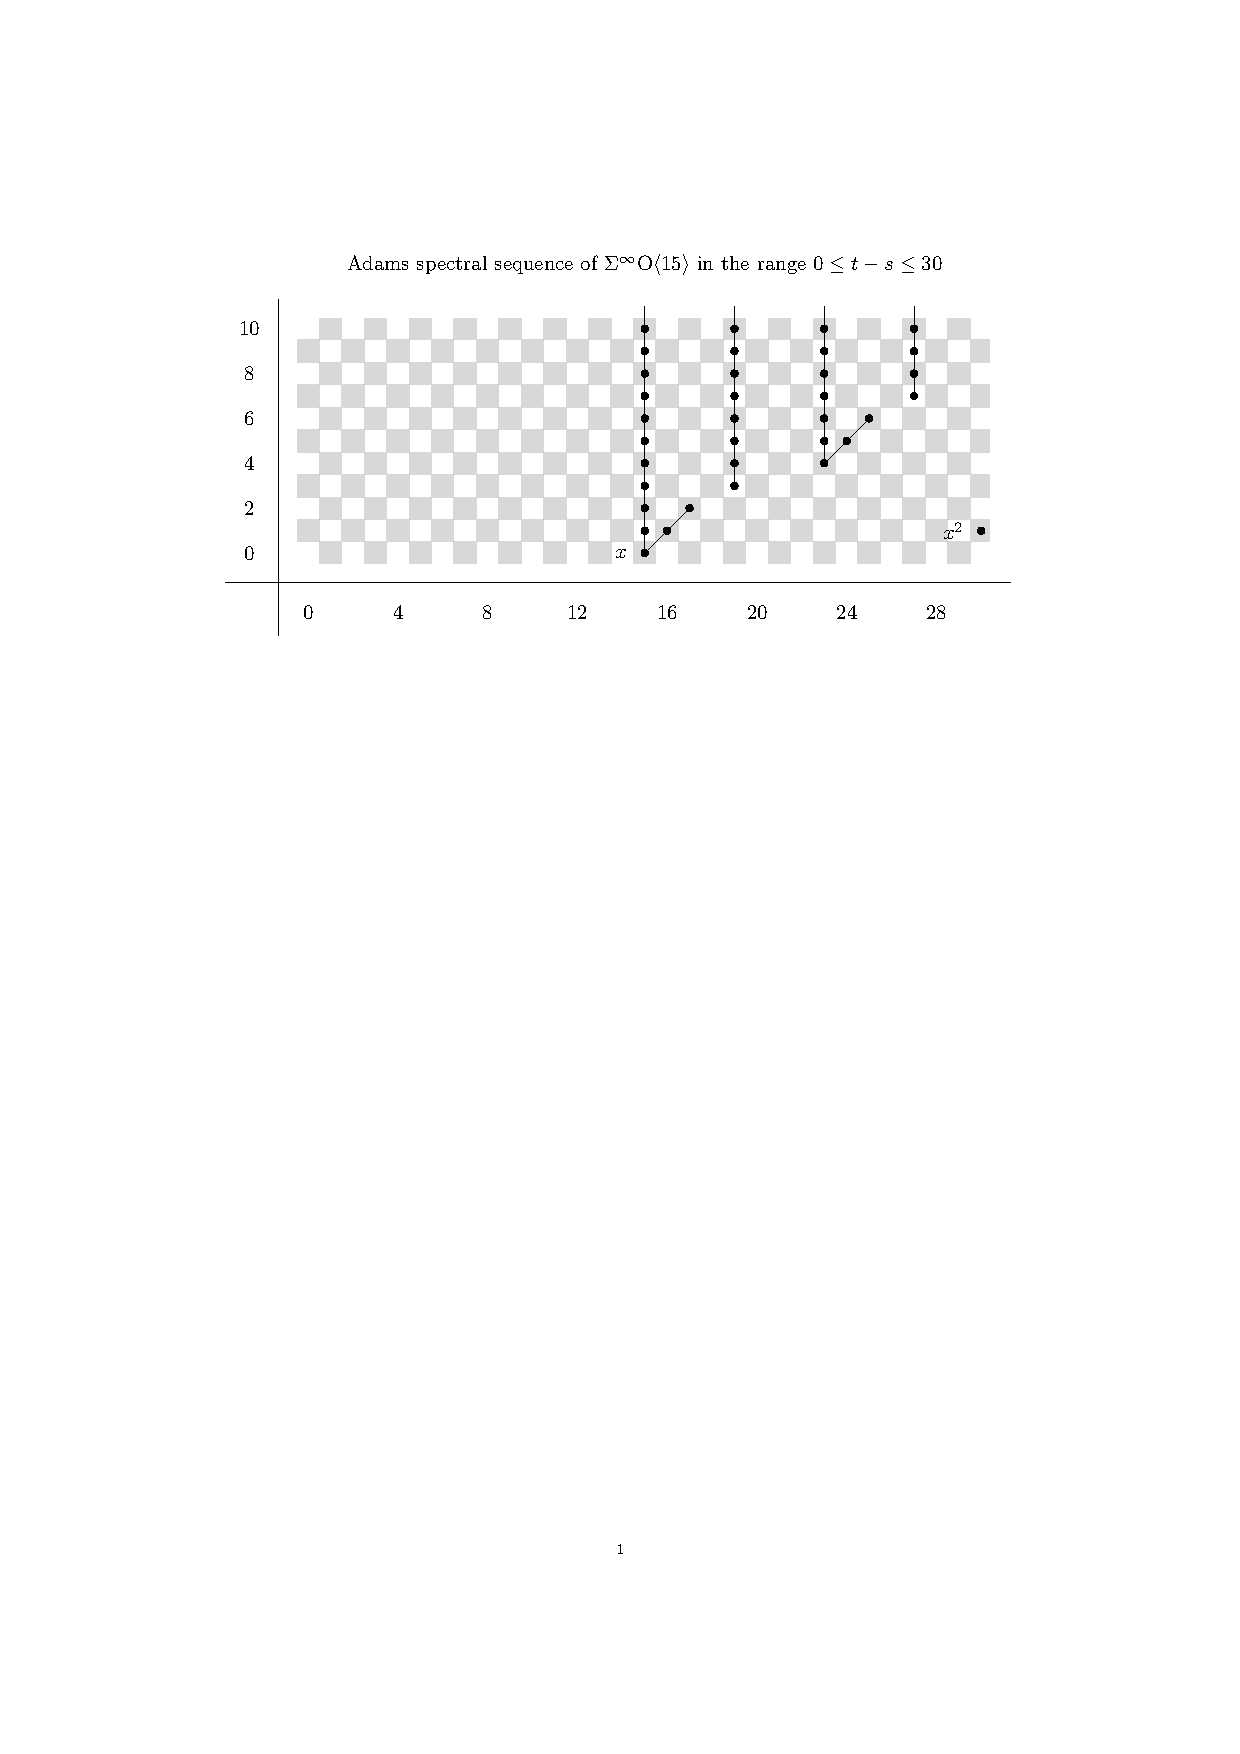
\includegraphics[trim={3.9cm 19cm 3.9cm 4.2cm}, clip, scale=1]{bleh3.pdf}
\end{figure}

\begin{proof}[Proof of \Cref{thm:vanishinggroup} when $p=2$]
  We will show that
  \[\pi_{8n-2, 8n-2+k} (\nu M) = 0\]
    for all $k \geq 2$, which is sufficient since $N_2 \geq 3$ for $n \geq 3$. Since $M$ is finite and implicitly $2$-completed, its $\HFt$-based Adams spectral sequence converges strongly \cite[Theorem 6.6]{BousfieldLocalization}, and we may apply \Cref{lemm:ctaugoodenough}. It therefore suffices to show that
  \[\pi_{8n-2, 8n-2+k} (C\tau \otimes \nu M ) = 0\]
  for all $k \geq 2.$ By \Cref{lemm:ctauE2}, 
  \begin{align*}
    \pi_{8n-2, 8n-2+k} (\nu M \otimes C\tau) &\cong \mathrm{E}_2 ^{k,8n-2+k} (M) \\
    &\cong \mathrm{E}_2 ^{k, 8n-2+k} (\Sigma^{\infty} \Oo \mathrm{\langle 4n-1 \rangle}),
  \end{align*}
  which is zero for $k \geq 2$ by \Cref{prop:E2compute}.
\end{proof}

%%% Local Variables:
%%% mode: latex
%%% eval: (visual-line-mode t)
%%% eval: (auto-fill-mode 0)
%%% End:
